\documentclass{article}
\title{Introduction to GeoDaSpace\footnote{First published: August/2012. Last revision: August/2012.}}
\author{}
\date{}
\usepackage{amsmath}
\usepackage{natbib}
\bibpunct{(}{)}{,}{a}{}{,}
\usepackage{float}
\usepackage{xcolor}
\usepackage{amssymb} 
\usepackage{listings}
\usepackage{caption}
\usepackage{hyperref}
\usepackage{subfig}
\usepackage{color,soul}
\usepackage[section]{placeins}
\usepackage{graphicx}
\graphicspath{{figures/}}
\DeclareCaptionFont{white}{\color{white}}
\DeclareCaptionFormat{listing}{%
  \parbox{\textwidth}{\colorbox{gray}{\parbox{\textwidth}{#1#2#3}}\vskip-4pt}}
\captionsetup[lstlisting]{format=listing,labelfont=white,textfont=white}
\lstset{frame=lrb,xleftmargin=\fboxsep,xrightmargin=-\fboxsep}
\newfloat{code}{H}{myc}

\begin{document}
\maketitle

\begin{figure}[htb]
\begin{center}

\includegraphics[width=0.5\linewidth]{geodaspace.png}\\
\end{center}
\end{figure}

\setcounter{secnumdepth}{3} 
\setcounter{tocdepth}{2}   
\tableofcontents
\newpage
%\listoffigures	
%\newpage
%\listoftables 

\section{Introduction}
\label{s:intro}

GeoDaSpace is a free software to estimate spatial regressions developed by the GeoDa Center for Geostatistical Analysis and Computation\footnote{For information on the GeoDa Center, please check \url{https://geodacenter.asu.edu}}. The software provides a graphical user interface (GUI) to the spatial regression module of PySAL (spreg)\footnote{More information on PySAL can be found at \url{http://pysal.geodacenter.org/}} \citep{Rey07}, an open source library for spatial analysis written in the object oriented language Python. The main estimation methods provided by GeoDaSpace are listed in Table \ref{t:methods}. As shown in the table, GeoDaSpace is a tool for the estimation of models of Ordinary Least Squares (OLS), Two-Stage Least Squares (TSLS), GMM spatial lag, GMM spatial error and GMM spatial lag and error, including both the method proposed by \citet{Kelejian98,Kelejian99} (KP98/99) and \citet{Drukker10} (KPD). All these estimation methods provide options for spatial and non-spatial diagnostics, non-spatial endogenous variables and the treatment of heteroskedasticity using HAC or White corrections, when applicable. In addition to these, GeoDaSpace offers a wide range of utilities to create and manipulate weights matrices, including contiguity, distance (bands, knn, inverse distance) and kernel.

Table \ref{t:methods} also shows the methods provided in GeoDaSpace that can be found in Stata and R. For this document we consider two different versions of the R package sphet. The first one, henceforth sphet1, is the released version of sphet (v. 1.1-12, published on CRAN on 2012-04-13). In addition to this version of sphet, we also use the alpha version from R-Forge, revision 56, published on 2012-07-22. This newer version of the code, which contains many additional methods and enhancements to sphet1, is henceforth referred as sphet2\footnote{Given that it is an alpha version, the code is subject to change.}.


\begin{table}[htpb]
\caption{Methods provided by GeoDaSpace and their availability in Stata or R}
\label{t:methods}
\centering
\begin{small}
\begin{tabular}{l|cccc} \hline
\textbf{Method}&\textbf{GeoDaSpace}&\textbf{Stata}&\textbf{R$^1$}&\textbf{R$^2$}\\ \hline
OLS&{\LARGE$\textcolor{blue}\bullet$}&{\LARGE$\textcolor{blue}\bullet$}&{\LARGE$\textcolor{blue}\bullet$}&{\LARGE$\textcolor{blue}\bullet$}\\
OLS with heteroskedasticity (White)&{\LARGE$\textcolor{blue}\bullet$}&{\LARGE$\textcolor{blue}\bullet$}&{\LARGE$\textcolor{blue}\bullet$}&{\LARGE$\textcolor{blue}\bullet$}\\
OLS with heteroskedasticity (HAC)&{\LARGE$\textcolor{blue}\bullet$}&&{\LARGE$\textcolor{blue}\bullet$}&{\LARGE$\textcolor{blue}\bullet$}\\
TSLS&{\LARGE$\textcolor{blue}\bullet$}&{\LARGE$\textcolor{blue}\bullet$}&{\LARGE$\textcolor{blue}\bullet$}&{\LARGE$\textcolor{blue}\bullet$}\\
TSLS with heteroskedasticity (White)&{\LARGE$\textcolor{blue}\bullet$}&{\LARGE$\textcolor{blue}\bullet$}&{\LARGE$\textcolor{blue}\bullet$}&{\LARGE$\textcolor{blue}\bullet$}\\
TSLS with heteroskedasticity (HAC)&{\LARGE$\textcolor{blue}\bullet$}&&{\LARGE$\textcolor{blue}\bullet$}&{\LARGE$\textcolor{blue}\bullet$}\\
Spatial lag&{\LARGE$\textcolor{blue}\bullet$}&{\LARGE$\textcolor{blue}\bullet$}&{\LARGE$\textcolor{blue}\bullet$}&{\LARGE$\textcolor{blue}\bullet$}\\
Spatial lag with het. (White)&{\LARGE$\textcolor{blue}\bullet$}&{\LARGE$\textcolor{blue}\bullet$}&{\LARGE$\textcolor{blue}\bullet$}&{\LARGE$\textcolor{blue}\bullet$}\\
Spatial lag with het. (HAC)&{\LARGE$\textcolor{blue}\bullet$}&&{\LARGE$\textcolor{blue}\bullet$}&{\LARGE$\textcolor{blue}\bullet$}\\
Spatial lag with endogenous var.&{\LARGE$\textcolor{blue}\bullet$}&{\LARGE$\textcolor{blue}\bullet$}&&{\LARGE$\textcolor{blue}\bullet$}\\
Spatial lag with endog. var. and het. (White)&{\LARGE$\textcolor{blue}\bullet$}&{\LARGE$\textcolor{blue}\bullet$}&&{\LARGE$\textcolor{blue}\bullet$}\\
Spatial lag with endog. var. and het. (HAC) &{\LARGE$\textcolor{blue}\bullet$}&&&{\LARGE$\textcolor{blue}\bullet$}\\
Spatial error (KP98/99)&{\LARGE$\textcolor{blue}\bullet$}&{\LARGE$\textcolor{blue}\bullet$}&{\LARGE$\textcolor{blue}\bullet$}&{\LARGE$\textcolor{blue}\bullet$}\\
Spatial error with endogenous var. (KP98/99)&{\LARGE$\textcolor{blue}\bullet$}&{\LARGE$\textcolor{blue}\bullet$}&&\\
Spatial error and lag (KP98/99)&{\LARGE$\textcolor{blue}\bullet$}&{\LARGE$\textcolor{blue}\bullet$}&{\LARGE$\textcolor{blue}\bullet$}&{\LARGE$\textcolor{blue}\bullet$}\\
Spatial error and lag w/ endog. var. (KP98/99)&{\LARGE$\textcolor{blue}\bullet$}&{\LARGE$\textcolor{blue}\bullet$}&&\\
Spatial error (KPD)&{\LARGE$\textcolor{blue}\bullet$}&{\LARGE$\textcolor{blue}\bullet$}&&{\LARGE$\textcolor{blue}\bullet$}\\
Spatial error with endogenous var. (KPD)&{\LARGE$\textcolor{blue}\bullet$}&{\LARGE$\textcolor{blue}\bullet$}&&{\LARGE$\textcolor{blue}\bullet$}\\
Spatial error and lag (KPD)&{\LARGE$\textcolor{blue}\bullet$}&{\LARGE$\textcolor{blue}\bullet$}&&{\LARGE$\textcolor{blue}\bullet$}\\
Spatial error and lag with endog. var. (KPD)&{\LARGE$\textcolor{blue}\bullet$}&{\LARGE$\textcolor{blue}\bullet$}&&{\LARGE$\textcolor{blue}\bullet$}\\
Spatial error with heteroskedasticity&{\LARGE$\textcolor{blue}\bullet$}&{\LARGE$\textcolor{blue}\bullet$}&{\LARGE$\textcolor{blue}\bullet$}&{\LARGE$\textcolor{blue}\bullet$}\\
Spatial error with endog. var. and het.&{\LARGE$\textcolor{blue}\bullet$}&{\LARGE$\textcolor{blue}\bullet$}&&{\LARGE$\textcolor{blue}\bullet$}\\
Spatial error and lag with het.&{\LARGE$\textcolor{blue}\bullet$}&{\LARGE$\textcolor{blue}\bullet$}&{\LARGE$\textcolor{blue}\bullet$}&{\LARGE$\textcolor{blue}\bullet$}\\
Spatial error and lag w/ endog. var. and het.&{\LARGE$\textcolor{blue}\bullet$}&{\LARGE$\textcolor{blue}\bullet$}&&{\LARGE$\textcolor{blue}\bullet$}\\
\hline
\multicolumn{5}{l}{\scriptsize{$^1$Considering the packages spdep and sphet (v. 1.1-12, published on CRAN on 2012-04-13).}} \\
\multicolumn{5}{l}{\scriptsize{$^2$Considering the packages spdep and sphet (revision 56, published on R-Forge on 2012-07-22).}} \\
\end{tabular}
\end{small}
\end{table}

The remainder of this document provides a basic introduction to the use of GeoDaSpace (Section \ref{s:GS}) . In addition to this, Section \ref{s:comparisons} presents a comparison of the estimation results using GeoDaSpace, Stata and R and explains the differences, when they occur. 

\newpage
\section{Using GeoDaSpace}
\label{s:GS}
\subsection{Opening a data file and specifying a model}

GeoDaSpace is a stand-alone software that provides a graphical user interface (GUI) to the spatial regression module of PySAL (spreg). It is available in Windows and Mac OSx versions.  The executable file can be downloaded for free from GeoDaCenter's website: \url{https://geodacenter.asu.edu/software}. 

The main GUI window is shown in Figure \ref{f:gui}. It can be divided in four sections: the menu icons (top), data and weights utilities (left), model specification (right) and model estimation (bottom). 

\begin{figure}[htb]
\caption{GeoDaSpace -- Main window}
\label{f:gui}
\begin{center}
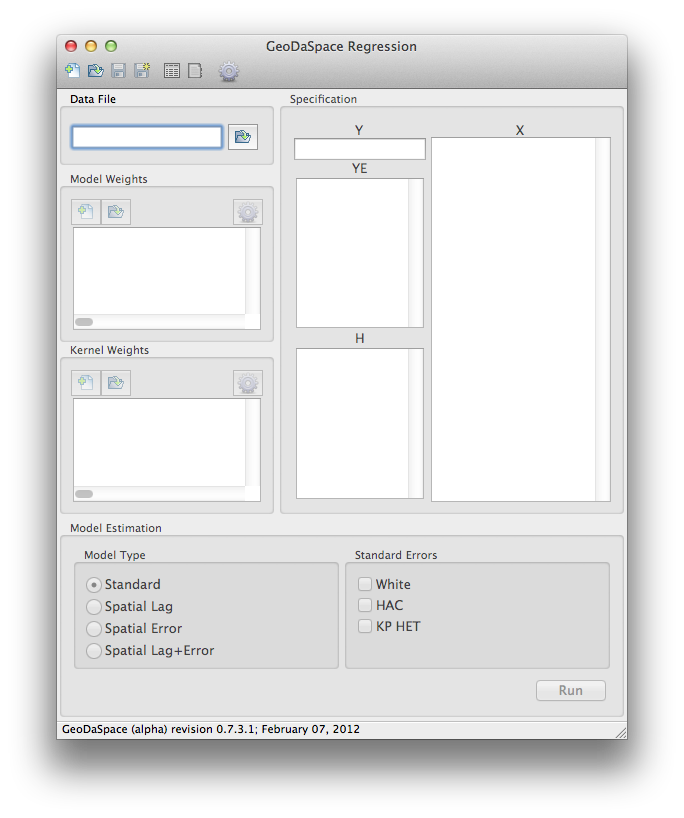
\includegraphics[width=0.8\linewidth]{GUI.png}\\
\end{center}
\end{figure}

The menu icons on the top of the window, from left to right, are:
\begin{itemize}
\item Create new model
\item Open existing model
\item Save model
\item Save model as...
\item Open the variables list
\item Show results window
\item Show advanced settings (see Section \ref{s:adv})
\end{itemize}

To start the specification of a new model, we need first to open the file containing the data. This can be done wither by clicking on the first menu icon `Create new model' or by clicking on the open folder icon within the data file section, as shown in Figure \ref{f:opendb}.

\begin{figure}[htb]
\caption{GeoDaSpace -- Open data file}
\label{f:opendb}
\begin{center}
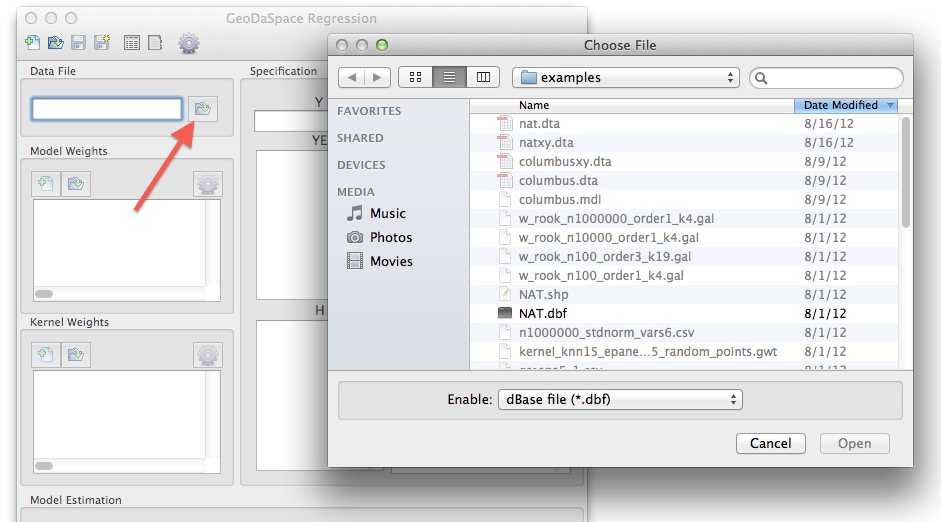
\includegraphics[width=0.9\linewidth]{opendb.png}\\
\end{center}
\end{figure}

Currently, GeoDaSpace can open data files in DBF, CSV and TXT formats. For the examples in this document, we use the NAT.dbf file\footnote{The data used in this document is available from PySAL's example data sets. It can be downloaded at \url{http://code.google.com/p/pysal/source/browse/\#svn\%2Ftrunk\%2Fpysal\%2Fexamples}}. Once we open the data file, its variables are listed in a side window. This window can be retrieved at any time by clicking on the fifth menu icon `Open the variable list'. To specify the model, click and drag the variables’ name from the list to the respective boxes in the Specification section of the main window (Figure \ref{f:spec}). The biggest box to the right, `X' (required), must contain all independent variables of the model, or the right-hand side variables. The other boxes are `Y' (required), for the dependent or left-hand side variable, `YE' (optional), which should be used in case there are endogenous explanatory variables, and `H' (optional), where the instruments for these endogenous explanatory variables should be specified.

\begin{figure}[htb]
\caption{GeoDaSpace -- Model specification}
\label{f:spec}
\begin{center}
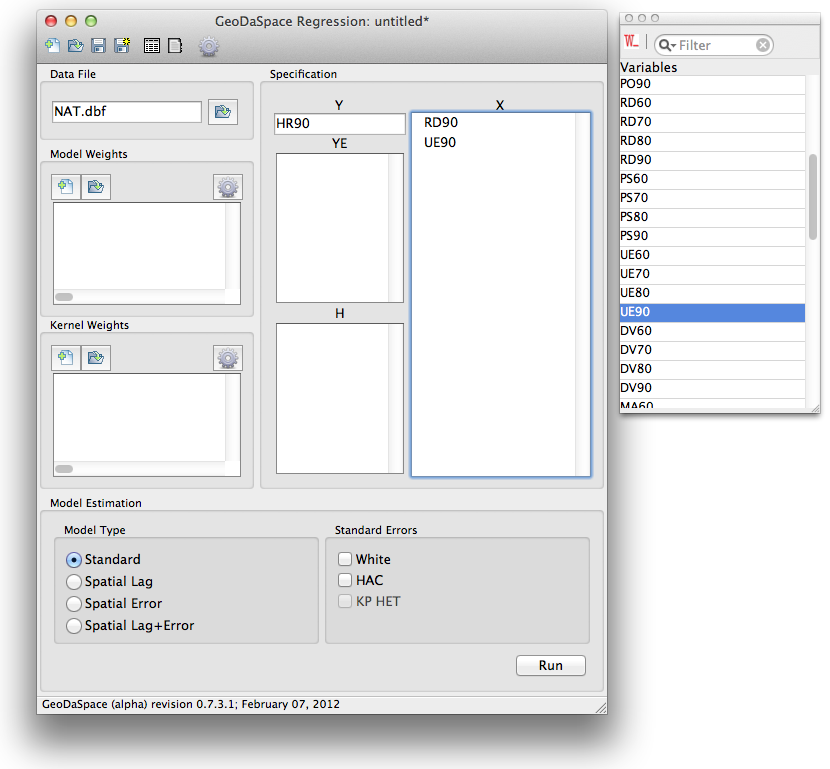
\includegraphics[width=0.9\linewidth]{spec.png}\\
\end{center}
\end{figure}
\FloatBarrier

\subsection{Weights creation}

In the weights section, it is possible to create a new weights matrix or open an existing one. GeoDaSpace supports most of the common weights formats, including GAL, GWT and KWT (GeoDa weights), MAT (MatLab), TXT (Stata Text files), among others. To create a new weights matrix we need to select the respective shapefile (SHP)\footnote{NAT.shp is available from PySAL's example data sets. It can be downloaded at \url{http://code.google.com/p/pysal/source/browse/\#svn\%2Ftrunk\%2Fpysal\%2Fexamples}} as `Input File' (Figure \ref{f:weights}). An ID variable for the weights matrix can either be selected from the database or added to it by clicking on the `plus' sign. GeoDaSpace can create standard model weights or kernel weights, each type with their respective boxes in the Weights section of the main window. Within standard model weights, GeoDaSpace can create contiguity weights matrices of the Queen and Rook types, for any given order of contiguity, according to the spatial structure of the shapefile. Distance weights are also available (Figure \ref{f:weights}a). Euclidean and Arc distances can be used as distance metrics. The types of distance weights available are: k-nearest neighbors, binary distance band and inverse distance. For the last two it is possible to select the cut-off point and, in the case of inverse distance, the power. If, for example, we want to create distance weights based on the inverse of the quadratic distance, all we have to do is choose `Distance' when creating a new weights matrix, then check the `Inverse Distance' bullet and set the power to 2 (Figure \ref{f:weights}a). The cut-off points establish the maximum distance between neighbors. If the metric is `Arc distance (miles)’ and the cut-off is 100, no spatial unit farther than 100 miles from each other will be considered neighbors. The default cut-off point is calculated to ensure that all spatial units have at least 1 neighbor, thus preventing the creation of units with no neighbors, i.e. islands.

\begin{figure}[htb]
\centering
\caption{GeoDaSpace -- Weights creation}
\label{f:weights}
\subfloat[Model weights]{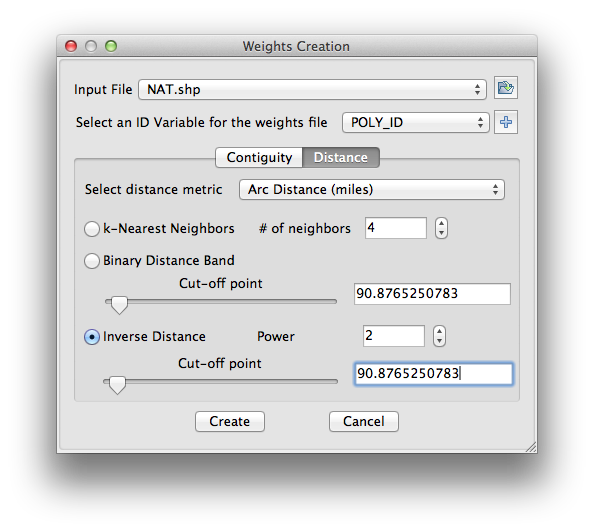
\includegraphics[width=0.5\textwidth]{distw.png}} 
\subfloat[Kernel weights]{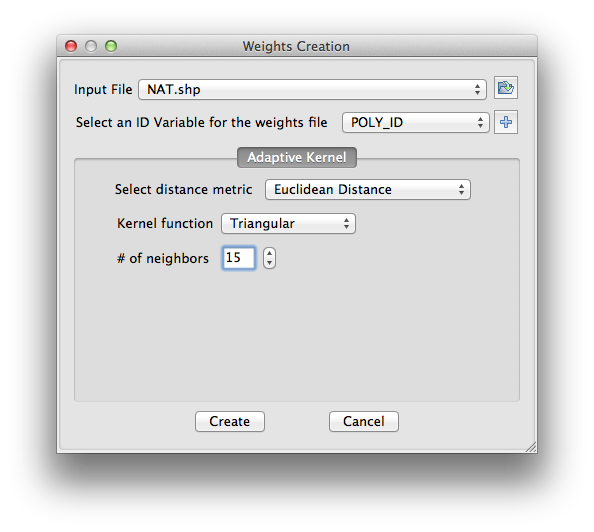
\includegraphics[width=0.5\textwidth]{kernel.png}} \\
\end{figure}

In addition to standard model weights, kernel weights can also be created (Figure \ref{f:weights}b). In GeoDaSpace, these are mainly used for the estimation of HAC models. Once again, Euclidean and Arc distances can be used as distance metrics. Currently, five Kernel functions are available: Uniform, Triangular, Epanechnikov, Quartic and Gaussian. It is also possible to specify the number of neighbors of each spatial unit.

The gear icon on the weights section opens a window showing the properties of the selected weights matrix. In this window, it is possible to transform the weights matrix into binary, row-standardized (each row summing 1), double-standardized (all row summing 1) and variance stabilized. The properties also include a list of the spatial units that have no neighbors, i.e. the islands, a list of the neighbors of any selected unit, the number of neighbors of each unit, i.e. the cardinalities, the unit's IDs and a histogram of units according to number of neighbors. As an experimental feature, it is also possible to launch an interactive viewer displaying the neighborhood structure. Within the viewer, we can pass the mouse arrow over any spatial unit of the shapefile and its neighbors are instantly highlighted. Also, their IDs are listed along with their weights (Figure \ref{f:viewer}).

\begin{figure}[htb]
\caption{GeoDaSpace -- Weights viewer}
\label{f:viewer}
\begin{center}
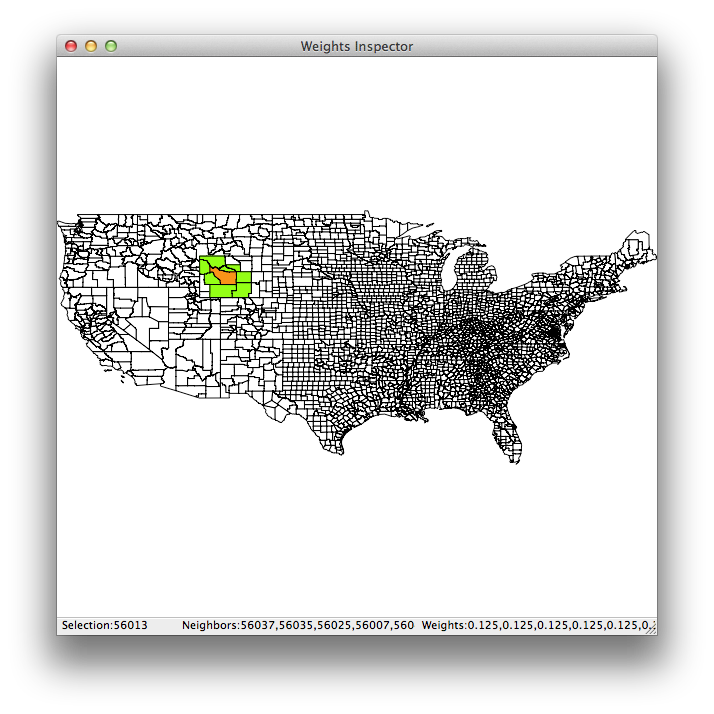
\includegraphics[width=\linewidth]{viewer.png}\\
\end{center}
\end{figure}
\FloatBarrier

\subsection{Model estimation}
The estimation methods available in GeoDaSpace can be selected from the `Model Estimation' section of the main window. There are four main model types: i) standard, ii) spatial lag, iii) spatial error and iv) spatial lag and error.

\subsubsection*{Standard}
\begin{itemize}
\item Ordinary least squares (OLS)
\item OLS with heteroskedasticity -- White
\item OLS with heteroskedasticity -- HAC
\item Two-stage least squares (TSLS)
\item TSLS with heteroskedasticity -- White
\item TSLS with heteroskedasticity -- HAC
\end{itemize}

\begin{figure}[htb]
\caption{Estimation of a TSLS model}
\label{f:tsls}
\begin{center}
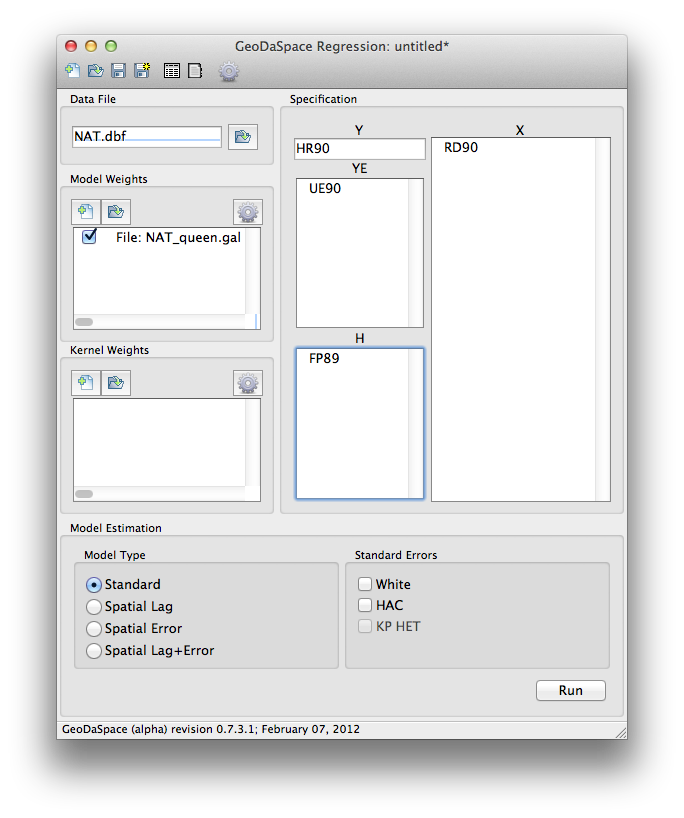
\includegraphics[width=0.7\linewidth]{tsls.png}\\
\end{center}
\end{figure}

The standard model types are OLS and TSLS models. These methods provide non-spatial diagnostics and spatial diagnostics, if a spatial weights matrix has been selected. In case there is no variable in the box `YE', implying the absence of any explanatory endogenous variable, an OLS model is estimated. If instead there is any variable in the box `YE', a TSLS is estimated. In this case, it is also required to provide in the box `H' the instruments for the endogenous variable (Figure \ref{f:tsls}). White and HAC (requires kernel weights) corrections for heteroskedasticity are available for these methods. The `KP HET' robust estimator assumes a spatial error structure, and therefore is not available for standard model types. Please see Section \ref{s:adv} for details on advanced settings for these methods.
\FloatBarrier

\subsubsection*{Spatial lag}
\begin{itemize}
\item Spatial lag
\item Spatial lag with heteroskedasticity -- White
\item Spatial lag with heteroskedasticity -- HAC
\item Spatial lag with additional endogenous variables
\item Spatial lag with additional endogenous variables and heteroskedasticity -- White
\item Spatial lag with additional endogenous variables and heteroskedasticity -- HAC
\end{itemize}

\begin{figure}[htb]
\caption{Estimation of a spatial lag model with heteroskedasticity -- HAC}
\label{f:haclag}
\begin{center}
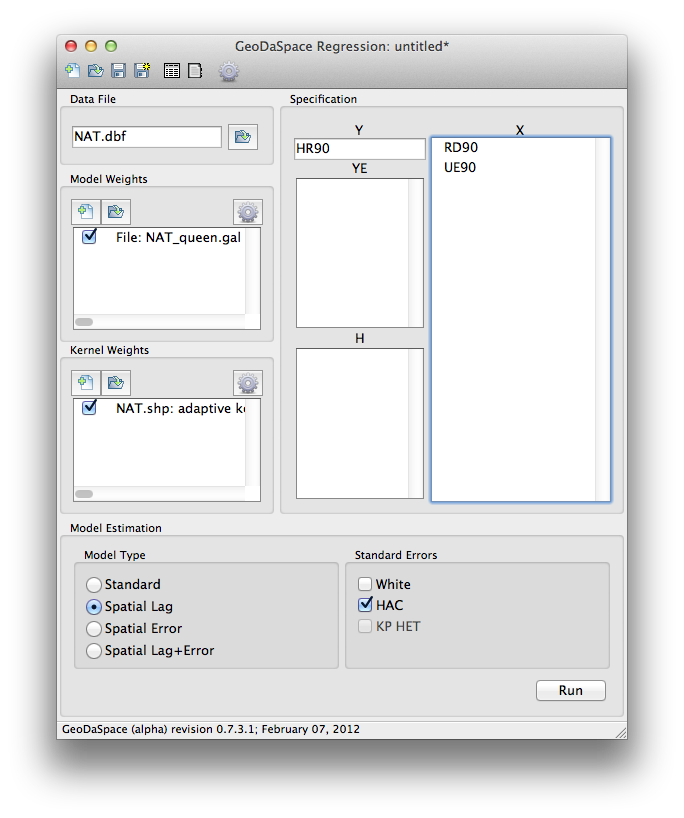
\includegraphics[width=0.7\linewidth]{haclag.png}\\
\end{center}
\end{figure}

The spatial lag type of model includes a lag of the dependent variable `Y' on the right side of the equation:
\begin{equation}
\mathbf{y} =  \rho \mathbf{W} \mathbf{y} + \mathbf{X}\beta + \varepsilon,
\end{equation}
or, alternatively:
\begin{equation}
\mathbf{y} =  (I - \rho \mathbf{W})^{-1} (\mathbf{X}\beta + \varepsilon),
\end{equation}
in which $\mathbf{y}$ is a $n \times 1$ vector containing the dependent variable `Y', $\mathbf{W}$ is the $n \times n$ spatial weights matrix, $\rho$ is the spatial autoregressive scalar parameter, $\mathbf{X}$ is a $n \times k$ matrix of observations on the explanatory variables `X', $\beta$ is a $k \times 1$ vector of coefficients, and $\varepsilon$ is a $n \times 1$ vector of random errors.

As with the standard methods, White and HAC (requires kernel weights) corrections for heteroskedasticity are available for spatial lag models. Figure \ref{f:haclag} shows an example of the estimation of a spatial lag model using HAC to correct the heteroskedasticity. The `KP HET' robust estimator is not available for models with spatial lag and no spatial errors, since it assumes a spatial error structure. Please see Section \ref{s:adv} for details on advanced settings for these methods.
\FloatBarrier

\subsubsection*{Spatial error}
\begin{itemize}
\item Spatial error (KPD)
\item Spatial error with endogenous variables (KPD)
\item Spatial error (KP98/99)
\item Spatial error with endogenous variables (KP98/99)
\item Spatial error with heteroskedasticity
\item Spatial error with endogenous variables and heteroskedasticity
\end{itemize}

\begin{figure}[htb]
\caption{Estimation of spatial error models with heteroskedasticity}
\label{f:GS_het}
\begin{center}
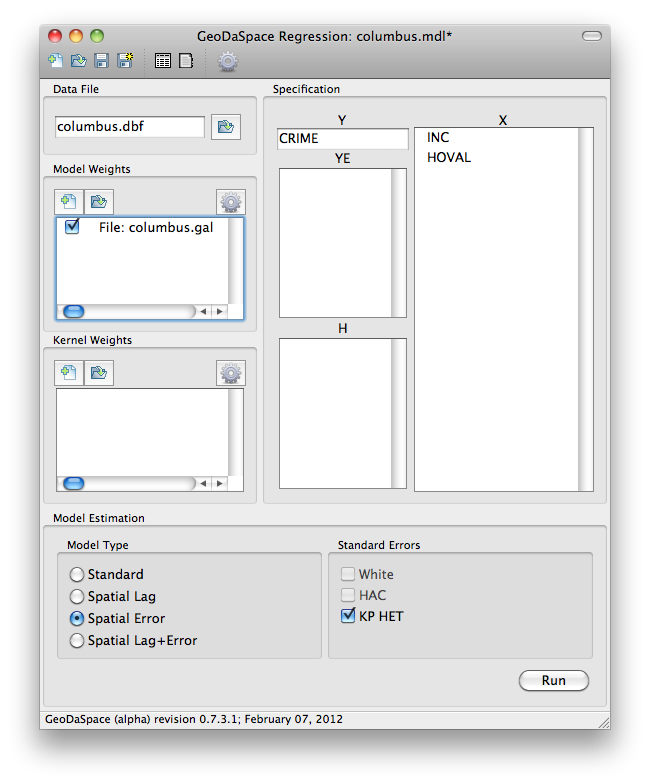
\includegraphics[width=0.7\linewidth]{GS_het.png}\\
\end{center}
\end{figure}

The spatial error type of model estimates a spatial autoregressive parameter in the errors ($\lambda$):
\begin{equation}
\mathbf{y} =  \mathbf{X}\beta + \mathbf{u},
\end{equation}
\begin{equation}
\mathbf{u} =  \lambda \mathbf{W} \mathbf{u} + \varepsilon,
\end{equation}
or, alternatively:
\begin{equation}
\mathbf{y} =  \mathbf{X}\beta + (I - \lambda \mathbf{W})^{-1} \varepsilon.
\end{equation}

GeoDaSpace provides two different estimators for spatial error models without heteroskedasticity. The default is the estimator proposed by \citet{Drukker10}, which we refer to as `KPD'. The second option is the estimator proposed by \citet{Kelejian98,Kelejian99}, here referred as `KP98/99'. The choice of the estimator to be used can be changed in the Advanced Settings Panel (Section \ref{s:adv}). Given the spatial structure of the error term, it is not possible to use White or HAC corrections for heteroskedasticity. Instead, GeoDaSpace can estimate the method proposed by \citet{Arraiz10}, which is robust to heteroskedasticity. To estimate this method, all we need to do is check both `Spatial Error' model type and `KP HET' standard errors (Figure \ref{f:GS_het}) Please see Section \ref{s:adv} for details on advanced settings for these methods.
\FloatBarrier

\subsubsection*{Spatial lag and error}
\begin{itemize}
\item Spatial lag and error (KPD)
\item Spatial lag and error with additional endogenous variables (KPD)
\item Spatial lag and error (KP98/99)
\item Spatial lag and error with additional endogenous variables (KP98/99)
\item Spatial lag and error with heteroskedasticity
\item Spatial lag and error with additional endogenous variables and heteroskedasticity
\end{itemize}

The spatial lag and error type of model estimates spatial autoregressive parameters both in the errors ($\lambda$) and for the spatial lag of the dependent variable ($\rho$):
\begin{equation}
\mathbf{y} = \rho \mathbf{W} \mathbf{y} + \mathbf{X}\beta + \mathbf{u},
\end{equation}
\begin{equation}
\mathbf{u} =  \lambda \mathbf{W} \mathbf{u} + \varepsilon,
\end{equation}
or, alternatively:
\begin{equation}
\mathbf{y} =  (I - \rho \mathbf{W})^{-1} \mathbf{X}\beta + (I - \rho \mathbf{W})^{-1}(I - \lambda \mathbf{W})^{-1} \varepsilon.
\end{equation}


\begin{figure}[htb]
\centering
\caption{Estimation of spatial lag and error model with heteroskedasticity}
\label{f:GS_het_combo}
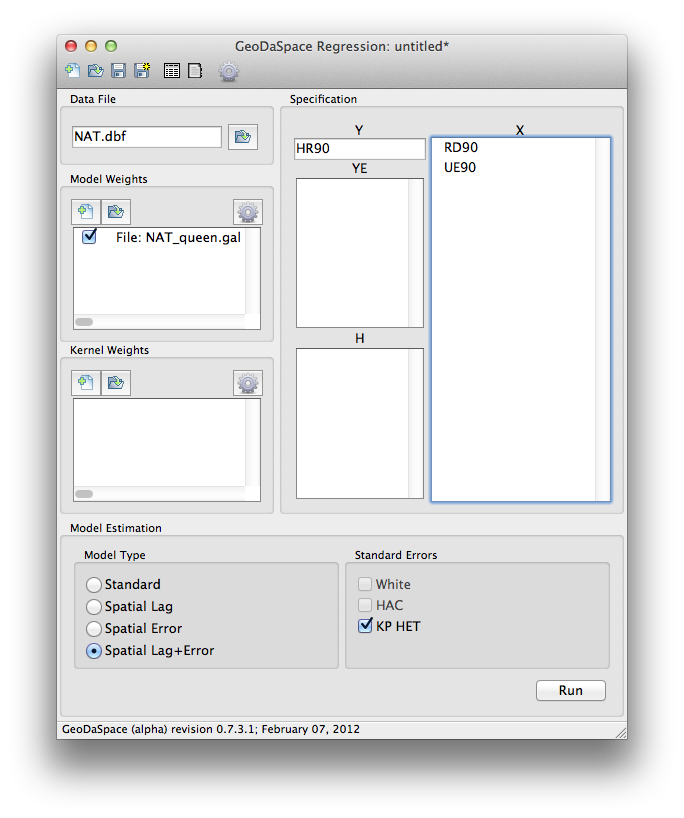
\includegraphics[width=0.7\textwidth]{GS_het_combo.png}
\end{figure}

All estimation methods for spatial error are also available in the presence of both spatial lag and spatial error. Once again, the default is the `KPD', but the `KP98/99' can be selected from the Advanced Settings Panel (Section \ref{s:adv}). In the presence of heteroskedasticity, it is possible to estimate the method proposed by \citet{Arraiz10} by checking both `Spatial Lag+Error' model type and `KP HET' standard errors. Figure \ref{f:GS_het_combo} shows how to estimate a spatial error model with spatial lag and heteroskedasticity in GeoDaSpace.
\FloatBarrier


\subsection{Advanced settings}
\label{s:adv}


The advanced contains several preferences that affect the way the methods implemented in GeoDaSpace are estimated. To access this panel, click on the gear icon on the top menu. (Figure \ref{f:gui_adv}).
 
\begin{figure}[htb]
\centering
\caption{Advanced settings panel}
\label{f:gui_adv}
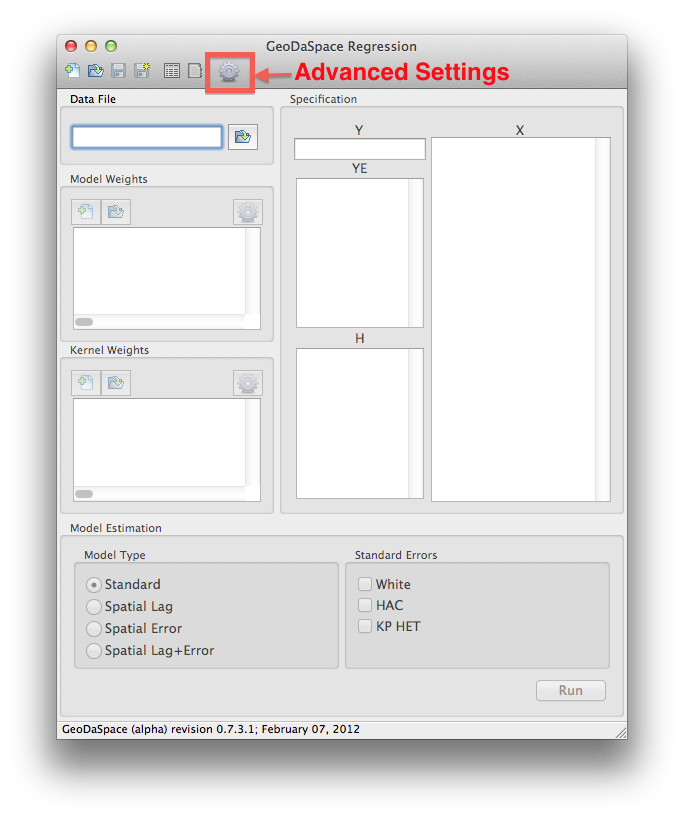
\includegraphics[width=0.9\textwidth]{GUI_adv.png}
\end{figure}
\FloatBarrier

\begin{figure}[htb]
\centering
\caption{Advanced settings panel -- Standard Deviations}
\label{f:adv_std}
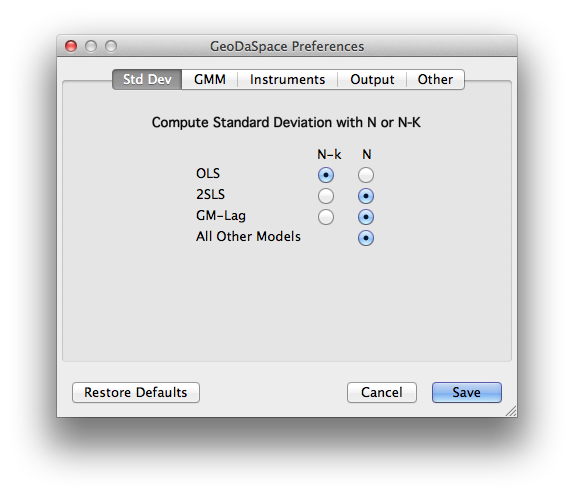
\includegraphics[width=0.7\textwidth]{adv_std.png}
\end{figure}

The first tab of the advanced settings panel is related to the way GeoDaSpace computes the standard deviation for all methods (Figure \ref{f:adv_std}). The formula for the normalization used in the calculation of the standard deviations can be selected for the OLS, TSLS, spatial lag and all other models. By default, only in the OLS case the denominator is $(N-k)$. Fall all others, the default is $N$. Of course, if $N$ is very large, the difference between both choices is insignificant. However, the results for small samples will vary according to the methodology selected.
\FloatBarrier

\begin{figure}[htb]
\centering
\caption{Advanced settings panel -- GMM}
\label{f:adv_gmm}
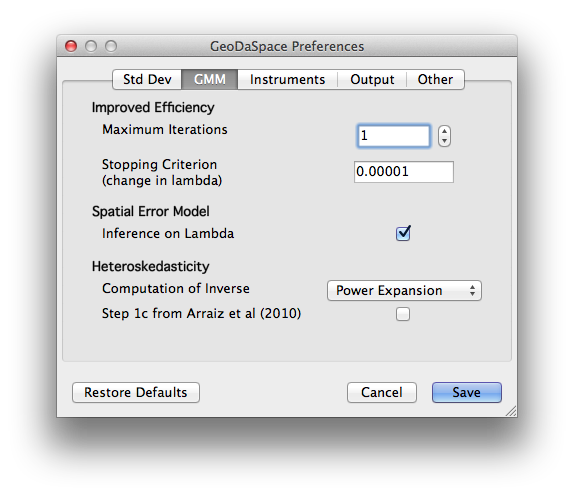
\includegraphics[width=0.7\textwidth]{adv_gmm.png}
\end{figure}

The second tab is related to the estimation of the GMM methods (Figure \ref{f:adv_gmm}). Estimators such as the KPD spatial error model \citep{Drukker10} and spatial error with heteroskedasticity KP-HET \citep{Arraiz10} allow for several iterations to improve efficiency (see \citet{Anselin11} for details). The maximum number of iterations can be selected in this tab, as well as the convergence criterion. When the difference between two subsequent estimations of $\lambda$ is less or equal than the value assigned in the box, no more iterations are performed. 

The second item in this tab refers to the inference on $\lambda$ in spatial error or spatial lag and error models. When there is no heteroskedasticity, this box defines if the estimation method selected is the KP98/99 or the KPD. The default, when the box is checked, provides the inference on $\lambda$ by estimating the KPD model. As originally proposed by \citet{Kelejian98,Kelejian99}, the estimation of the KP98/99 does not provide this inference. The KP98/99 is the method used when the box is unchecked.

The third and last item in the GMM tab is related to the estimation of spatial error models with heteroskedasticity. Here we can select the method for the computation of the inverse of the operations involving the $\mathbf{W}$ matrix. By default, a power expansion is performed in these cases, so that the computational time is decreased. If instead the true inverse is desired, this option is available from the drop-down list. In addition to this, we can also opt for having step 1c in the estimation of the spatial error model with heteroskedasticity, as proposed by \citet{Arraiz10}. Step 1c updates the initial consistent estimation of lambda using a weighted nonlinear least squares solution to the moments equations. This results in a consistent and efficient intermediate estimation of $\lambda$. Note however that a consistent estimation at this stage is already sufficient to obtain a consistent estimation of all parameters in the model. For this reason, the default in GeoDaSpace is to skip this step to save computational time.
\FloatBarrier

\begin{figure}[htb]
\centering
\caption{Advanced settings panel -- Instruments}
\label{f:adv_inst}
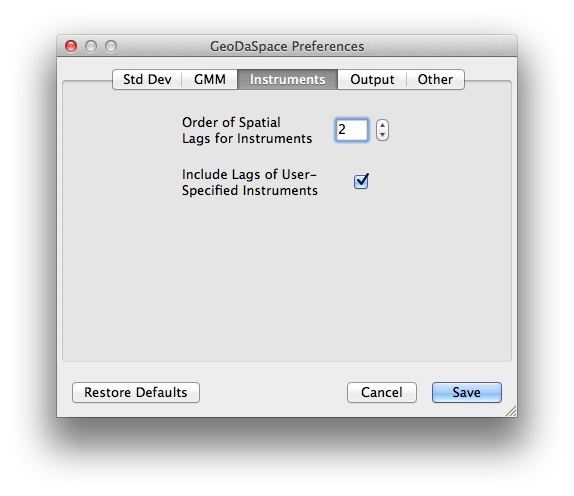
\includegraphics[width=0.7\textwidth]{adv_inst.png}
\end{figure}

The third tab is the Instruments tab (Figure \ref{f:adv_inst}). In this tab it is possible to change the way GeoDaSpace deals with instruments in case of a spatial lag or spatial lag and error models. The first item refers to the order of the spatial lags of the exogenous variables used as instruments of the spatial lag of the dependent variable. The default is to have first and second order lags of these variables, i.e. $\mathbf{WX} + \mathbf{W^2X}$, as instruments to $\mathbf{Wy}$. If instead we change the order of spatial for 1, we have that only $\mathbf{WX}$ will be used as instruments. 

The second checkbox, checked by default, determines the inclusion of the spatial lag of the user-specified instruments in addition to the lag of the exogenous variables. Of course, this applies only if additional instruments are provided in the instruments box `H’ on the main GUI. The instruments in this case are $\mathbf{WX} + \mathbf{W^2X} + \mathbf{WH} + \mathbf{W^2H}$.
\FloatBarrier

\begin{figure}[htb]
\centering
\caption{Advanced settings panel -- Output}
\label{f:adv_out}
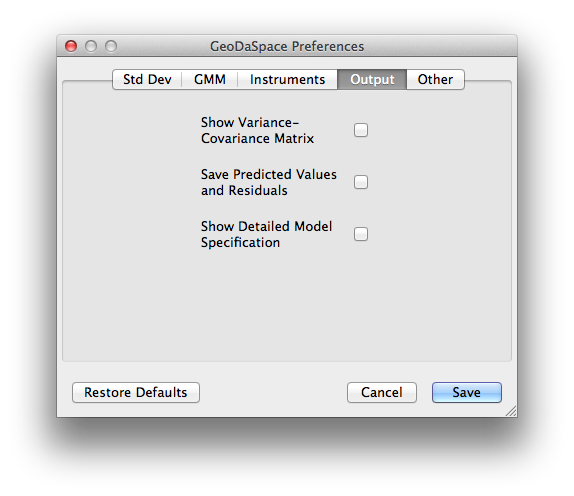
\includegraphics[width=0.7\textwidth]{adv_out.png}
\end{figure}
\FloatBarrier

The fourth tab is related to the output that is printed by GeoDaSpace in the results window (Figure \ref{f:adv_out}).  The first checkbox controls the printing of the $k \times k$ variance-covariance matrix of the estimated parameters. When the box is checked (default), the variance-covariance matrix will be displayed below the estimation main results.

The second item allows us to save the predicted values of the dependent variable and residuals in a spreadsheet. If this option is checked, GeoDaSpace creates a CSV files containing this information. Before the estimation is performed, a pop-up window allows us to choose the folder and filename.

The last item in the Output box is ``Show Detailed Model Specification’’. This option is currently unavailable and checking it will not affect the output.

The last tab contains other type of options. Its first item refers to the calculation of regression diagnostics. By default, non-spatial diagnostics are calculated when running an OLS model. These diagnostics include Jarque-Bera normality test, heteroskedasticity and multicollinearity diagnostics. Another item is related to the calculation of the Moran’s I test for spatial dependence. Whenever a spatial matrix is selected when running standard models, LM tests will be calculated and their results will be printed on the results window. When the box for the Moran’s I is check in the advanced settings panel, the Moran’s I is also included. By default this option is disabled since the calculation of the Moran’s I slows the computation time, especially for large samples.

\begin{figure}[htb]
\centering
\caption{Advanced settings panel -- Other}
\label{f:adv_other}
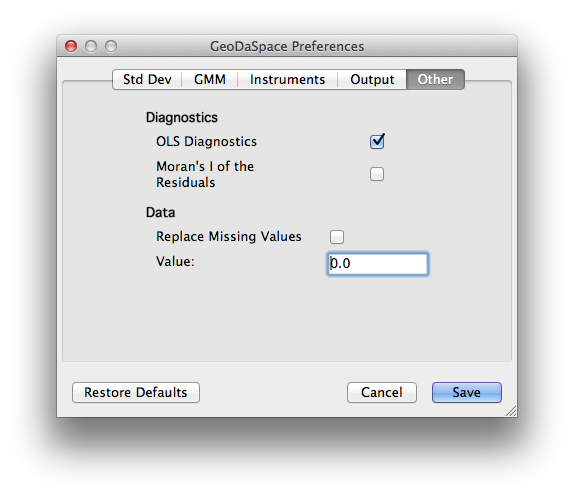
\includegraphics[width=0.7\textwidth]{adv_other.png}
\end{figure}

The second group of items in this tab refers to data manipulation. Currently GeoDaSpace cannot deal with missing values in the data. When these exist, this option allows us to replace all missing values by a given value (zero by default).

It is possible to save all options in the advanced settings panel. By clicking on the `Save’ button, these chosen options will be saved for future sessions of GeoDaSpace, not only for the model currently being estimated. It is also possible to restore the default values at any time by clicking on the respective button and then saving these changes.

\newpage

\section{Comparing estimation results from GeoDaSpace, Stata and R: reasons for difference and pathway for matching}
\label{s:comparisons}

\subsection{Introduction}
In this section we compare the results of models with spatial error from 3 different programs: GeoDaSpace, R and Stata. Despite all the methods available in GeoDaSpace (see Section \ref{s:intro}), here we show only those which yield discrepant results in GeoDaSpace in comparison with Stata. An explanation for the differences is provided. In addition, we show how to set the preferences in GeoDaSpace in order to get the same results from Stata. When this option is not available, we show how PySAL\footnote{More information on PySAL can be found at \url{http://pysal.geodacenter.org/}} \citep{Rey07}, a Python library on which GeoDaSpace is based, can be used to match Stata.

For this document we use two different versions of the R package sphet. The first one, henceforth sphet1, is the released version of sphet (v. 1.1-12, published on CRAN on 2012-04-13). In addition to this version of sphet, we also use the alpha version from R-Forge, revision 56, published on 2012-07-22. This newer version of the code, which contains many additional methods and enhancements to sphet1, is henceforth referred as sphet2\footnote{Given that it is an alpha version, the code is subject to change.}.


The following spatial error models (SEM) are discussed in this section:

\begin{itemize}
\item SEM with exogenous variables and no heteroskedasticity (KPD)
\item SEM with endogenous variables and no heteroskedasticity (KPD)
\item SEM with spatial lag and no heteroskedasticity (KPD)
\item SEM with exogenous variables and heteroskedasticity
\item SEM with endogenous variables and heteroskedasticity
\item SEM with spatial lag and heteroskedasticity
\end{itemize}

\subsection{Spatial Error Models without Heteroskedasticity}

The default spatial error model without heteroskedasticity in GeoDaSpace is the KPD model \citep{Drukker10}. Given the particular specification of the model when all variables as exogenous, as presented in \citet{Anselin11}, the results from GeoDaSpace do not match those from Stata when this method is used. This discrepancy is due to an error in Stata for the case of a spatial error model with exogenous variables only. In Stata, the exogeneity is ignored and a two-stage least squares estimation is performed instead of the OLS.

Table \ref{t:res_hom} compares the results from GeoDaSpace, Stata and R. The KPD method is not available in the currently released version of sphet1 (v. 1.1-12). Nonetheless, the results presented here can be obtained using sphet2, the alpha version from R-Forge. As Table \ref{t:res_hom} shows, the results from GeoDaSpace differ from those from sphet2. 

\begin{table}[htpb]
\caption{Comparison of the results of spatial error models with exogenous variables and no heteroskedasticity}
\label{t:res_hom}
\centering
\begin{small}
\begin{tabular}{l|cccc} \hline
\textbf{Variable}&\textbf{GeoDaSpace}&\textbf{sphet2}&\textbf{Stata}&\textbf{PySAL$^1$}\\ \hline
CONSTANT&8.0259&6.6762&6.9884&6.9884\\
&(0.3601)&(0.3498)&(0.3605)&(0.3605)\\
RD90&4.3228&3.9450&3.9945&3.9945\\
&(0.1596)&(0.1553)&(0.1612)&(0.1612)\\
UE90&-0.2753&-0.0770&-0.1240&-0.1240\\
&(0.0479)&(0.0471)&(0.0490)&(0.0490)\\
lambda&0.4572&0.4149&0.4124&0.4124\\
&(0.0189)&(0.0194)&(0.0194)&(0.0194)\\
\hline
\multicolumn{5}{l}{\scriptsize{$^1$PySAL using the code to match Stata as in Listing \ref{lt:hom_stata}.}} \\
\end{tabular}
\end{small}
\end{table}


Despite the problems with Stata's estimator, PySAL allows us to match its results. To do so, we have to use PySAL's Base classes, that allows us to specify the model more freely. Since Stata performs a 2SLS estimation, in order to match its results using PySAL we have to specify X as both the endogenous variables and the instruments. Since PySAL requires at least one exogenous variable, we create a constant to use as such. In addition to the different treatment given to exogenous variables in Stata, the A1 matrix used to estimate the model is also different. In GeoDaSpace's code, the option was for the use of the matrix proposed by \citet{Arraiz10} instead of \citet{Drukker10} and \citet{Drukker11}. The details of this choice can be found in \citet{Anselin11}. Listing \ref{lt:hom_stata} shows the command that will allow PySAL to match the results from Stata for the spatial error model\footnote{A walkthrough for the estimation of spatial error models without heteroskedasticity using PySAL can be found at \url{http://pysal.geodacenter.org/dev/library/spreg/error_sp_hom.html}}. 

\begin{code}
\begin{lstlisting}[label=lt:hom_stata,caption=Using PySAL to match the results of spatial error models from Stata,language=Python]

import pysal
import numpy as np

w = pysal.open('NAT_queen.gal').read()
w.transform = 'r'
db = pysal.open('NAT.dbf')
hr90 = np.array([db.by_col('HR90')]).T
rd90 = np.array([db.by_col('RD90')]).T
ue90 = np.array([db.by_col('UE90')]).T
x = np.hstack((rd90,ue90))

ones = np.ones(crime.shape)
model = pysal.spreg.BaseGM_Endog_Error_Hom(hr90, ones,
        yend=x, q=x, w=w, A1='hom_sc')

print model.betas
print map(np.sqrt, model.vm.diagonal())

\end{lstlisting}
\end{code}

If we have endogenous variables, or a spatial lag, the problem in Stata's code no longer exists, since we now do have to run a 2SLS estimator. Nonetheless, the results from GeoDaSpace remain different from those from Stata and R, as shown in Table \ref{t:res_hom_endog}. The diffence is due to the choice of the A1 matrix used in the estimations and, for the spatial lag, the number of lags of the exogenous variables used as instruments.  

\begin{table}[htpb]
\caption{Comparison of the results of spatial error models with endogenous variables or spatial lag}
\label{t:res_hom_endog}
\centering
\begin{small}
\begin{tabular}{l|cccc} \hline
\multicolumn{5}{c}{\textbf{Spatial error with UE90 as endogenous variable}} \\ \hline
\textbf{Variable}&\textbf{GeoDaSpace}&\textbf{sphet2}&\textbf{Stata}&\textbf{PySAL$^1$}\\ \hline
CONSTANT&21.0288&19.7052&21.0606&21.0606\\
&(1.5362)&(1.4194)&(1.5385)&(1.5385)\\
RD90&8.2376&8.0369&8.2420&8.2420\\
&(0.4881)&(0.4634)&(0.4888)&(0.4888)\\
UE90$^2$&-2.2392&-2.0396&-2.2438&-2.2438\\
&(0.2286)&(0.2111)&(0.2290)&(0.2290)\\
lambda&0.4934&0.4856&0.4944&0.4944\\
&(0.0216)&(0.0220)&(0.0217)&(0.0217)\\
\hline
\multicolumn{5}{c}{\textbf{Spatial error with spatial lag}} \\ \hline
\textbf{Variable}&\textbf{GeoDaSpace$^3$}&\textbf{sphet2}&\textbf{Stata}&\textbf{PySAL$^1$}\\ \hline
CONSTANT&6.9406&6.9362&6.9362&6.9362\\
&(0.5327)&(0.5120)&(0.5120)&(0.5120)\\
RD90&4.0074&4.0061&4.0061&4.0061\\
&(0.1758)&(0.1764)&(0.1764)&(0.1764)\\
UE90&-0.0957&-0.0978&-0.0978&-0.0978\\
&(0.0490)&(0.0481)&(0.0481)&(0.0481)\\
W\_HR90&-0.0220&-0.0190&-0.0190&-0.0190\\
&(0.0543)&(0.0513)&(0.0513)&(0.0513)\\
lambda&0.5098&0.4364&0.4364&0.4364\\
&(0.0376)&(0.0421)&(0.0421)&(0.0421)\\
\hline
\multicolumn{5}{l}{\scriptsize{$^1$PySAL using the code to match Stata as in Listing \ref{lt:hom_end_stata}.}} \\
\multicolumn{5}{l}{\scriptsize{$^2$UE90 instrumented by FP89 and all other exogenous variables.}} \\
\multicolumn{5}{l}{\scriptsize{$^3$GeoDaSpace using 2 spatial lags for the instruments.}} \\
\multicolumn{5}{l}{\scriptsize{\hl{Note:I'm still not convinced I'm doing the endog model in R right.}}} \\
\multicolumn{5}{l}{\scriptsize{\hl{I'll have to check with Gianfranco. He says he's results match Stata's.}}} \\
\end{tabular}
\end{small}
\end{table}

Once again, PySAL offers the possibility of matching Stata. As shown in Listing \ref{lt:hom_end_stata}, all that we have to do is to select the option `hom\_sc' for the argument A1. By doing so, we override the default A1=`het', in which the matrix A1 is defined as in \citet{Arraiz10} by opting for the A1 as used in Stata and presented in \citet{Drukker10} and \citet{Drukker11}. For the case of a spatial lag, it is also important to set the amount of spatial lags of the exogenous variables to be used as instrument of the spatial lag of the dependent variable. The default used in GeoDaSpace is `1'. The value must be changed to `2' in order to match Stata's results. The code shown in Listing \ref{lt:hom_end_stata} continues from Listing \ref{lt:hom_stata}.

\begin{code}
\begin{lstlisting}[label=lt:hom_end_stata,caption=Using PySAL to match the results of spatial error models with endogenous variables or spatial lag from Stata,language=Python]

#Spatial error model with spatial lag:
model = pysal.spreg.GM_Combo_Hom(hr90, x, w=w, 
        A1='hom_sc', w_lags=2)
print model.summary

#Adding instrument 'FP89':
fp89 = np.array([db.by_col('FP89')]).T

#Spatial error model with UE90 as endogenous variable:
model = pysal.spreg.GM_Endog_Error_Hom(hr90, rd90,
        yend=ue90, q=fp89, w=w, A1='hom_sc')
print model.summary

\end{lstlisting}
\end{code}

\subsection{Spatial Error Models with Heteroskedasticity}

As in the case with no heteroskedasticity, Stata's code has an error in the estimation of the spatial error model with exogenous variables only. Therefore, it is not possible to match the results from Stata for this specification using GeoDaSpace. Table \ref{t:res_het} compares GeoDaSpace's results against Stata and the package sphet from R. As already stated, we refer to the released version 1.1-12 of sphet as sphet1 and the updated alpha version of spreg available from R-Forge (revision 56 published on 2012-07-22) is referred as sphet2. Differently than sphet2, the version sphet1 does not allow us to skip one step in the estimation of the method (step1c), which is done by default in GeoDaSpace, Stata and sphet2. Please check Section \ref{s:step1c} for more details on this.

\begin{table}[htpb]
\caption{Comparison of the results of spatial error models with exogenous variables and heteroskedasticity}
\label{t:res_het}
\centering
\begin{small}
\begin{tabular}{l|ccccc} \hline
\textbf{Variable}&\textbf{GeoDaSpace}&\textbf{sphet1}&\textbf{sphet2}&\textbf{Stata}&\textbf{PySAL$^1$}\\ \hline
CONSTANT&6.6586&6.5782&6.6586&6.9777&6.9777\\
&(0.4749)&(0.4594)&(0.4745)&(0.4622)&(0.4622)\\
RD90&3.9417&3.9275&3.9417&3.9911&3.9911\\
&(0.2602)&(0.2316)&(0.2599)&(0.2326)&(0.2325)\\
UE90&-0.0745&-0.0630&-0.0745&-0.1225&-0.1225\\
&(0.0611)&(0.0589)&(0.0611)&(0.0592)&(0.0592)\\
lambda&0.4753&0.4756&0.4740&0.4721&0.4721\\
&(0.0235)&(0.0237)&(0.0237)&(0.0236)&(0.0236)\\
\hline
\multicolumn{6}{l}{\scriptsize{$^1$PySAL using the code to match Stata as in Listing \ref{lt:het_stata}.}} \\
\end{tabular}
\end{small}
\end{table}

In PySAL, it is possible to mimic the problem in Stata's code to estimate a model that yields the same results\footnote{A walkthrough for the estimation of spatial error models with heteroskedasticity using PySAL can be found at \url{http://pysal.geodacenter.org/dev/library/spreg/error_sp_het.html}}. The code is shown in Listing \ref{lt:het_stata}.

\begin{code}
\begin{lstlisting}[label=lt:het_stata,caption=Using PySAL to match the results of spatial error models with heteroskedasticity from Stata,language=Python]

import pysal
import numpy as np

w = pysal.open('NAT_queen.gal').read()
w.transform = 'r'
db = pysal.open('NAT.dbf')
hr90 = np.array([db.by_col('HR90')]).T
rd90 = np.array([db.by_col('RD90')]).T
ue90 = np.array([db.by_col('UE90')]).T
x = np.hstack((rd90,ue90))

model = pysal.spreg.BaseGM_Endog_Error_Het(hr90, ones,
        yend=x, q=x, w=w)

print model.summary

\end{lstlisting}
\end{code}

When the spatial error model with heteroskedasticity contains a spatial lag, the default specification in GeoDaSpace does match the results from Stata. This is due to the order of the spatial lags of the exogenous variables used as instruments of the spatial lag of the dependent variable. The default in GeoDaSpace is a single lag. In Stata however the model is run lagging the exogenous variables twice. This option cannot be changed in Stata. In GeoDaSpace, we can choose the number of lags desired from the Preferences Panel (see Section \ref{s:adv}). If we select `2' as the order of spatial lags for instruments, the results from GeoDaSpace match Stata's, as shown in Table \ref{t:res_het_combo}. 
\begin{table}[htpb]
\caption{Comparison of the results of spatial error models with spatial lag and heteroskedasticity}
\label{t:res_het_combo}
\centering
\begin{small}
\begin{tabular}{l|ccccc} \hline
\textbf{Variable}&\textbf{GeoDaSpace$^1$}&\textbf{sphet1}&\textbf{sphet2}&\textbf{Stata}&\textbf{PySAL$^2$}\\ \hline
CONSTANT&6.9406&7.0196&6.9406&6.9406&6.9406\\
&(0.8600)&(0.8251)&(0.8600)&(0.8600)&(0.8600)\\
RD90&4.0074&4.0057&4.0074&4.0074&4.0074\\
&(0.3261)&(0.3212)&(0.3261)&(0.3261)&(0.3261)\\
UE90&-0.0957&-0.0643&-0.0957&-0.0957&-0.0957\\
&(0.0664)&(0.0640)&(0.0664)&(0.0664)&(0.0664)\\
W\_HR90&-0.0220&-0.0702&-0.0220&-0.0220&-0.0220\\
&(0.0876)&(0.0839)&(0.0876)&(0.0876)&(0.0876)\\
lambda&0.5584&0.6399&0.5584&0.5584&0.5584\\
&(0.0507)&(0.0460)&(0.0507)&(0.0507)&(0.0507)\\
\hline
\multicolumn{6}{l}{\scriptsize{$^1$GeoDaSpace using 2 spatial lags for the instruments.}} \\
\multicolumn{6}{l}{\scriptsize{$^2$PySAL using the code to match Stata as in Listing \ref{lt:het_endog_stata}.}} \\
\end{tabular}
\end{small}
\end{table}

If the spatial error model with heteroskedasticity contains other type of endogenous variables, but not a spatial lag, the results from GeoDaSpace match those from Stata without the need of any change (Table \ref{t:res_het_endog}).

\begin{table}[htpb]
\caption{Comparison of the results of spatial error models with endogenous variable (UE90) and heteroskedasticity}
\label{t:res_het_endog}
\centering
\begin{small}
\begin{tabular}{l|cccc} \hline
\textbf{Variable}&\textbf{GeoDaSpace}&\textbf{sphet2$^1$}&\textbf{Stata}&\textbf{PySAL$^2$}\\ \hline
CONSTANT&21.0288&19.6812&21.0288&21.0288\\
&(2.5629)&(2.2653)&(2.5629)&(2.5629)\\
RD90&8.2376&8.0401&8.2376&8.2376\\
&(0.7817)&(0.7161)&(0.7817)&(0.7817)\\
UE90$^3$&-2.2392&-2.0361&-2.2392&-2.2392\\
&(0.3902)&(0.3449)&(0.3902)&(0.3902)\\
lambda&0.4667&0.4614&0.4667&0.4667\\
&(0.0298)&(0.0295)&(0.0298)&(0.0298)\\
\hline
\multicolumn{5}{l}{\scriptsize{$^1$sphet1 does not allow for endogenous variables.}} \\
\multicolumn{5}{l}{\scriptsize{$^2$PySAL using the code to match Stata as in Listing \ref{lt:het_endog_stata}.}} \\
\multicolumn{5}{l}{\scriptsize{$^3$UE90 instrumented by FP89 and exogenous variables.}} \\
\multicolumn{5}{l}{\scriptsize{\hl{Note:I'm still not convinced I'm doing the endog model in R right.}}} \\
\multicolumn{5}{l}{\scriptsize{\hl{I'll have to check with Gianfranco. He says he's results match Stata's.}}} \\
\end{tabular}
\end{small}
\end{table}


In PySAL, these models could be estimated using the code shown in Listing \ref{lt:het_endog_stata}. This code is a continuation of Listing \ref{lt:het_stata}.

\begin{code}
\begin{lstlisting}[label=lt:het_endog_stata,caption=Using PySAL to match the results of spatial error models with heteroskedasticity and endogenous variables or spatial lag from Stata,language=Python]

#Spatial error model with spatial lag and
#    heteroskedasticity:
model = pysal.spreg.GM_Combo_Het(hr90, x,
        w=w, w_lags=2)
print model.summary

#Adding instrument 'FP89':
fp89 = np.array([db.by_col('FP89')]).T

#Spatial error model with UE90 as endogenous variable
#    and heteroskedasticity:
model = pysal.spreg.GM_Endog_Error_Het(hr90, rd90,
        yend=ue90, q=fp89, w=w)
print model.summary

\end{lstlisting}
\end{code}
\FloatBarrier


\subsubsection{Initial Efficient Estimation of Lambda (Step1c)}
\label{s:step1c}
In addition to the number of lags of the exogenous variables to be used as instruments, both GeoDaSpace and PySAL also offer the possibility to add the Step 1c in the estimation of the model as proposed by \citet{Arraiz10}. Step 1c updates the initial consistent estimation of lambda using a weighted nonlinear least squares solution to the moments equations. This results in a consistent and efficient intermediate estimation of lambda. Note however that a consistent estimation at this stage is already sufficient to obtain a consistent estimation of all parameters in the model. The option to run Step 1c can be found in the preferences panel in GeoDaSpace, as shown in Section \ref{s:adv}. In PySAL, all we have to do to select this option is add `step1c=True' to the arguments of the model (Listing \ref{lt:het_step1c}).

\begin{code}
\begin{lstlisting}[label=lt:het_step1c,caption=Using PySAL to match the results of spatial error models with heteroskedasticity and endogenous variables or spatial lag from Stata,language=Python]

#Spatial error model with heteroskedasticity
#    (running Step1c):
model = pysal.spreg.GM_Error_Het(hr90, x,
        w=w, step1c=True)
print model.summary

#Spatial error model with spatial lag and
#    heteroskedasticity (running Step1c):
model = pysal.spreg.GM_Combo_Het(hr90, x,
        w=w, step1c=True)
print model.summary

#Spatial error model with HOVAL as endogenous variable
#    and heteroskedasticity (running Step1c):
model = pysal.spreg.GM_Endog_Error_Het(hr90, rd90,
        yend=ue90, q=fp89, w=w, step1c=True)
print model.summary

\end{lstlisting}
\end{code}


\newpage
\bibliography{bib}
\bibliographystyle{apalike}
\end{document}




